\chapter{Implementace}
\section{Využité technologie}
Aplikace byla vytvořena za použití nástroje Microsoft Visual Studio 2019, což je populární vývojové prostředí (IDE) vyvíjené firmou Microsoft. Toto prostředí je, co se týče programování aplikací pro operační systém Windows vyvíjený stejnojmennou firmou, standardem. Také u naší aplikace se proto počítá s využitím zmíněného operačního systému k jejímu provozu. Využíván je také .NET Framework \cite{net-framework}, což je platforma sloužící vývojářům k vytváření a spouštění aplikací. Tato platforma má velké množství verzí, u této aplikace počítáme s využitím verze .NET Framework 4.7.2. Naší aplikaci bychom mohli kategorizovat jako aplikaci s grafickým uživatelským rozhraním (GUI), což je pojem známý spíše pod svým anglickým jménem „Windows Application“. Pro implementaci uživatelského rozhraní je v případě této aplikace využita knihovna tříd Windows Forms \cite{winforms}, která je také součástí .NET Frameworku. K naprogramování celé aplikace byl využit programovací jazyk C\#, což je objektově orientovaný jazyk vyvíjený taktéž firmou Microsoft.

\section{Objektová analýza}
Třídy obsažené v aplikaci bychom mohli podle jejich funkce rozdělit na dvě skupiny.
\begin{itemize}
	\item Ovládání hry
		\begin{itemize}
		\item \lstinline$Hra$
		\item \lstinline$PohybPocitacovehoHrace$
		\item \lstinline$VypocetMoznychTahu$
	\end{itemize}
	\item Herní entity
		\begin{itemize}
		\item \lstinline$LidskyHrac$
		\item \lstinline$MoznyTahLidskehoHrace$
		\item \lstinline$MoznyTahLPocitacovehoHrace$
		\item \lstinline$PocitacovyHrac$
		\item \lstinline$Pole$
		\item \lstinline$VychoziPolePocitacovehoHrace$
		\item \lstinline$ZvyrazneniPoleLidskehoHrace$
		\item \lstinline$ZvyrazneniPolePocitacovehoHrace$
	\end{itemize}
\end{itemize}

U některých entit bychom si mohli všimnout rozdělení na entity lidského a počítačového hráče. Tyto entity (tedy možný tah, pole hráče a zvýraznění pole) mají vlastní objekty a využívají vlastní kolekce, a to i přes to, že mají stejné nebo velmi podobné parametry i metody. Jistě by tedy šlo použít jediný objekt a jedinou kolekci pro všechny hráče a funkčnost aplikace by zůstala beze změny. Důvod pro jejich rozdělení je jednoduchý -– s entitami lidského a počítačových hráčů pracujeme vždy odděleně, takže rozdělení jejich objektů ve výsledku výrazně usnadní práci s těmito objekty. Pokud bychom objekty neoddělili, museli bychom při každé iteraci kolekce některé ze skupin objektů specifikovat, kterého hráče se daná iterace týká. Takový postup by vzhledem k vysokému počtu cyklů nacházejících se v programu značně ztížil jakoukoli manipulaci s danými objekty, a navíc by zde byl prostor k neúmyslnému vytváření obtížně vysledovatelných chyb.

Pro upřesnění je na obrázku \ref{fig:TridniDiagram} k dispozici třídní diagram celé aplikace. U tříd z kategorie \emph{Herní entity} bylo vzhledem k menšímu počtu parametrů a metod možné do diagramu zaznamenat vše, u tříd z kategorie \emph{Ovládání hry} jsou ale uvedeny jen některé (zpravidla nejdůležitější) parametry a metody. Pro úsporu místa jsou také v diagramu používány zkratky, například u třídy \lstinline$PohybPocitacovehoHrace$ namísto „PocitacovyHrac“ zapisujeme \enquote{PHrac}.

\begin{figure}
	\centering
	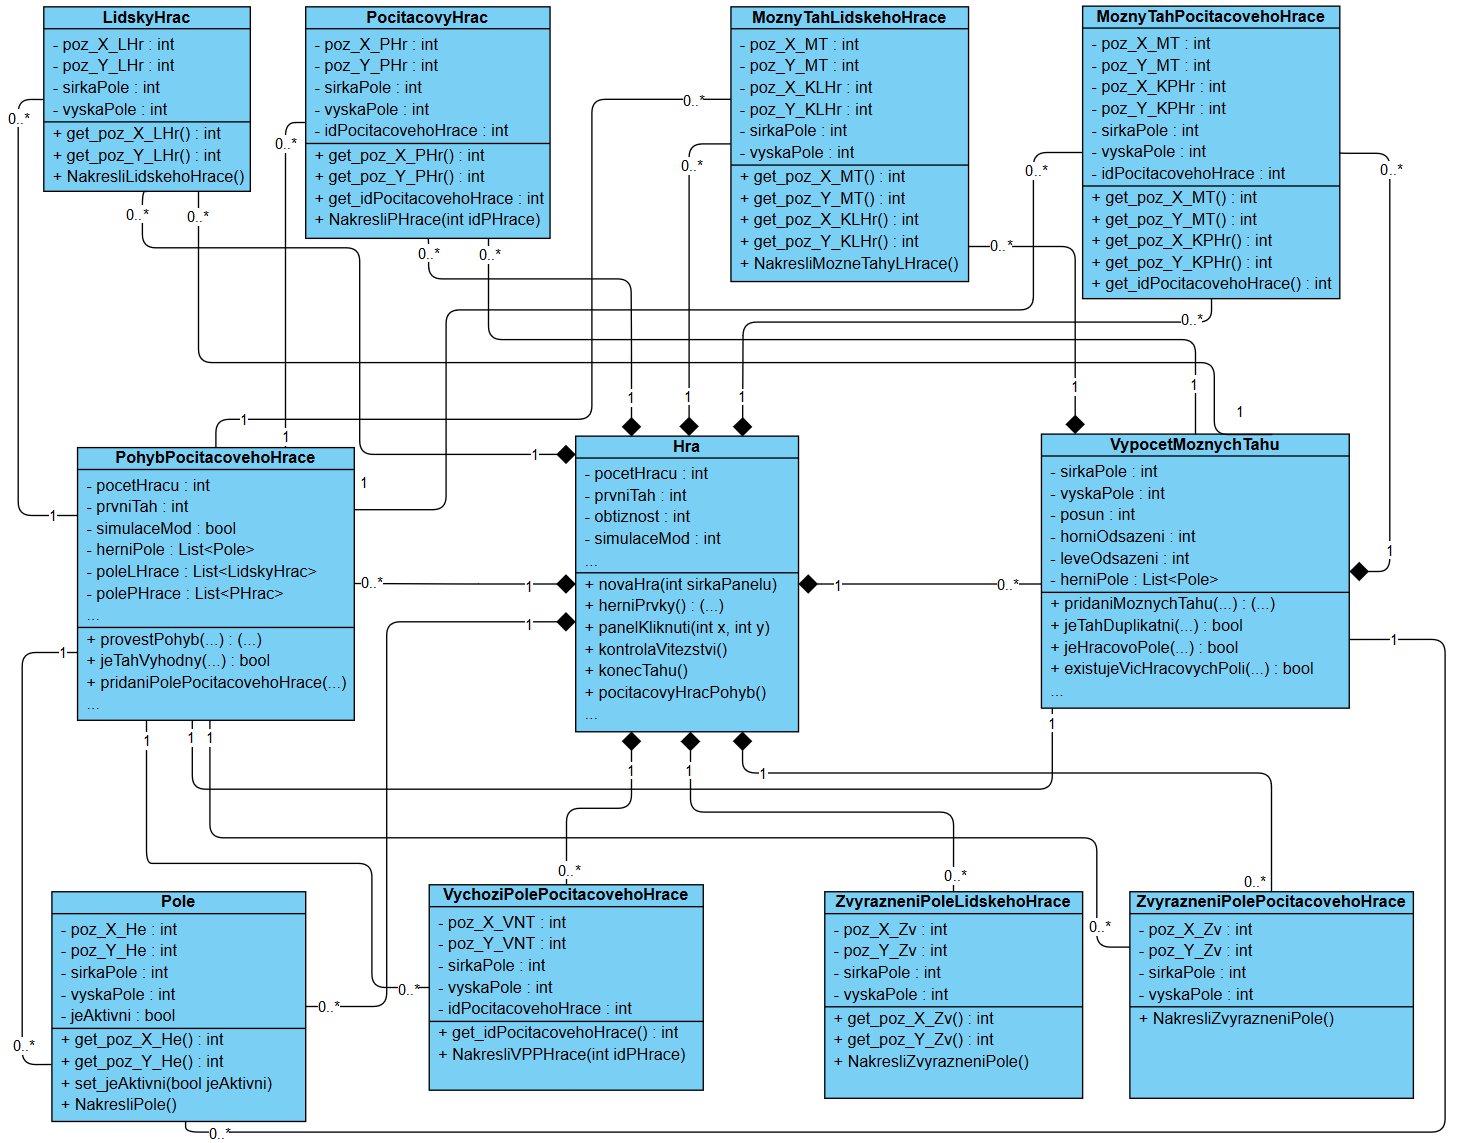
\includegraphics[width=1\textwidth]{Figures/TridniDiagram.png}
	\caption{Třídní diagram aplikace Čínská dáma}
    \label{fig:TridniDiagram}
\end{figure}

\section{Vytvoření a provoz hry}
\label{sec:VytvoreniAProvozHry}
Hra je vytvořena zavoláním metody \lstinline$NovaHra$ třídy \lstinline$Hra$. Toto volání probíhá v konstruktoru třídy \lstinline$HraForm$, což je třída, prostřednictvím které hráč ovládá hru a sleduje její aktuální stav. V konstruktoru je taktéž vytvářena instance třídy \lstinline$Hra$, přičemž jsou do třídy Hra předány parametry, které nastavuje uživatel. Předáván je tímto způsobem počet hráčů, dále informace o tom, jestli se jedná o simulaci a obtížnost počítačových hráčů. Mimo to si uživatel může také zvolit, jestli bude první na tahu on, nebo počítačový hráč (nabízí se i možnost vybrat začínajícího hráče náhodně, což by odpovídalo hodu mincí, který může být využíván k určení začínajícího hráče u her na fyzické herní desce). 

V metodě \lstinline$NovaHra$ nejprve dochází k vytvoření herní desky (tento proces je blíže vysvětlen v~podkapitole \ref{sec:HerniPole}). Po vytvoření herního pole jsou vytvořena pole lidského a počítačových hráčů. Každý hráč má unikátní ID, které je využíváno mimo jiné při kontrole vítězství u jednotlivých hráčů. Přidělování ID funguje na stejném principu jako přidělování barev, přidělováno je vždy na základě výchozího trojúhelníku hráče, nezávisle na počtu hráčů. Ukázku systému přidělování ID na základě výchozího trojúhelníku můžeme vidět na obrázku číslo \ref{fig:IDPocitacovychHracu}. Na zmíněném obrázku je k~modrému hráči přiděleno ID 0. Nejedná se o lidského hráče (který má přidělené ID 1), jedná se o~modrého počítačového hráče, který je ale využíván pouze při simulacích.

\begin{figure}
	\centering
	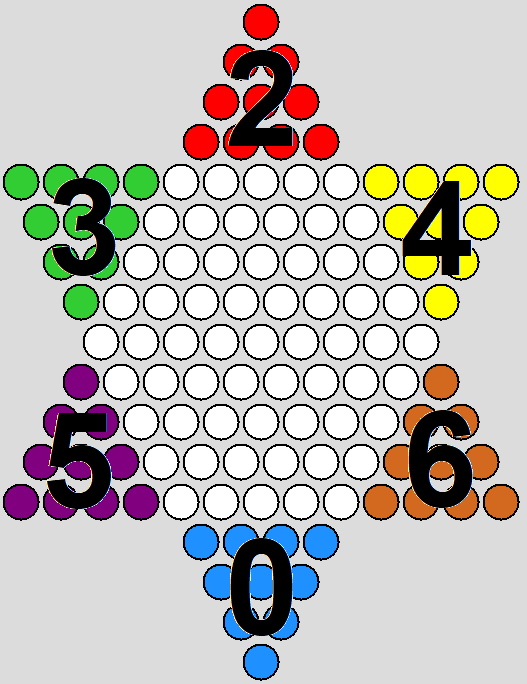
\includegraphics[width=0.4\textwidth]{Figures/IDPocitacovychHracu.png}
	\caption{Počítačoví hráči podle jejich ID}
    \label{fig:IDPocitacovychHracu}
\end{figure}

Hráči jsou vytvářeni na základě splnění podmínek. Jednak musí být pro jejich vytvoření nastaven odpovídající počet hráčů. Dále jsou v cyklu procházena všechna herní pole a probíhá kontrola, jestli se má na daném poli nacházet daný počítačový hráč. U hráčů v nejvýše a nejníže položeném trojúhelníku je tato kontrola velmi jednoduchá -– záleží pouze na $y$-ové poloze daného pole.~U~zbývajících čtyř hráčů je ale tato kontrola o poznání složitější -– záleží jak na $y$-ové poloze, tak na $x$-ové.

Pro umožnění znovupoužitelnosti a snadnější čitelnost kódu jsou tyto podmínky uloženy v metodě \lstinline$JePoleVHornimLevemRohu$, do které jsou vyslány souřadnice daného pole a je vrácena informace o tom, jestli se pole v daném trojúhelníku nachází nebo ne. Metody fungující na stejném principu jsou samozřejmě vytvořeny pro každý trojúhelník obsažený ve hvězdě.

Po vytvoření všech zmíněných polí je hra připravená. Hru ovládá uživatel (lidský hráč) kliknutím na některé ze svých herních polí a následně kliknutím na některý z možných tahů (průběh zpracování možných tahů je vysvětlen v následující podkapitole). Po dokončení hráčova tahu jsou na tahu počítačoví hráči. Je zavolána metoda \lstinline$KonecTahu$, ve které proběhne zavolání metody \lstinline$ProvestPohyb$ ve třídě \lstinline$PohybPocitacovehoHrace$, do které je posláno aktuální rozložení herní desky a jejímž návratovým typem je rozložení herní desky s novými pozicemi počítačových hráčů. Počítačoví hráči jsou v této metodě procházeni v cyklu a v každé iteraci je určen tah vždy jednoho počítačového hráče. 

\section{Vytvoření možných tahů}
\label{sec:VytvoreniMoznychTahu}
Jak už bylo zmíněno v podkapitole \ref{sec:MozneTahy}, aplikace podporuje tahy na sousední pole a skoky, pohyby je možné provádět v šesti směrech. V této podkapitole je prezentována implementace tahů na sousední pole a také skoku v jednom z šesti směrů. Postup vytvoření možných tahů a výběru některého z~nich by se dal shrnout v následujících bodech:
\begin{enumerate}
	\item Lidský hráč klikne na jeden ze svých kamenů
\item\label{moznyTahPostup} Aplikace zvýrazní daný kámen a světle modře vyznačí všechna pole, na která se hráč může přesunout
\item Lidský hráč si kliknutím vybere jedno z nabízených polí
	\item Aplikace po výběru pole vyhodnotí další postup
	\begin{enumerate}
		\item hráč si vybral sousední pole, jeho tah je ukončen
		\item hráč provedl skok, aplikace provede stejný postup jako v bodě \ref{moznyTahPostup}, hráč může provést libovolné množství skoků, tah poté ukončí kliknutím na zvýrazněné pole nebo na tlačítko v kontrolním panelu
	\end{enumerate}
	\item Tah lidského hráče skončil, aplikace odstraní kámen na původní poloze a vytvoří kámen na právě vybrané poloze, na tahu jsou nyní počítačoví hráči
\end{enumerate}

Když hráč klikne na jeden ze svých kamenů, jsou v metodě \lstinline$PanelKliknuti$ třídy \lstinline$Hra$ v cyklu procházena všechna herní pole, přičemž v každé iteraci je kontrolováno, jestli pole splňuje podmínky pro to, aby bylo přidáno jako možný tah. Na začátku každé iterace je ještě zkontrolováno, jestli se pole nenachází v jiném než výchozím nebo cílovém trojúhelníku daného hráče, do těchto polí totiž hráč nemá přístup. Nejprve budou prezentovány podmínky pro vytvoření možného tahu na sousedních polích. Podmínky i s vysvětlivkami jsou k dispozici ve výpisu číslo \ref{src:moznyTahSousedniPole}.

\begin{lstlisting}[label=src:moznyTahSousedniPole,caption={Podmínky pro vytvoření možného tahu - sousední pole}]
Math.Abs(poz_Y_KHr - poz_Y_He) <= posun /*vzdálenost kliknutého hráčova pole a právě procházeného herního pole není větší než dané odsazení mezi herními poli (na y-ové ose)*/ &&
Math.Abs(poz_X_KHr - poz_X_He) <= posun /*vzdálenost kliknutého hráčova pole a právě procházeného herního pole není větší než dané odsazení mezi herními poli (na x-ové ose)*/ &&
!JeTahDuplikatni(poz_X_He, poz_Y_He, poz_X_KHr, poz_Y_KHr, idHrace, mozneTahyLidskehoHrace, mozneTahyPocitacovehoHrace) /*tah není duplikátní (na daném poli se již nenachází možný tah daného hráče)*/ &&
!JeHracovoPole(poz_X_He, poz_Y_He, poleLidskehoHrace, polePocitacovehoHrace) /*na daném poli není žádné hráčovo nebo nepřítelovo pole*/ &&
!hracSePohlSkokem /*hráč neprovedl ve svém tahu skok -- tahy na sousední pole a skoky nelze během jednoho tahu kombinovat*/
\end{lstlisting}

Následují možné tahy vykonávané prostřednictvím skoků. Ty už jsou jak na porozumění, tak na implementaci složitější než tahy na sousední pole. Při provedení skoku je ve třídě Hra do proměnných \lstinline$delkaSkokuX$ a \lstinline$delkaSkokuY$ uložena délka skoku na $x$-ové, resp. $y$-ové ose. Jedná se o vzdálenost pole, na kterém se nacházel přesouvaný kámen a pole, na které byl kámen přemístěn na daných osách. Při skoku je také nastavena proměnná \lstinline$hracProvedlSkok$ na \lstinline$true$, což je využito k zamezení přidání sousedních polí jako možných tahů po provedení skoku. V metodě \lstinline$PridaniMoznychTahu$ už v cyklu neprocházíme pouze herní pole (jako u tahů na sousední pole), ale také pole lidského a počítačových hráčů, protože právě tato pole jsou během skoků přeskakována. Pro příklad budou prezentovány pouze skoky v nevodorovném směru, tedy skoky, u kterých je délka skoku na $y$-ové ose vyšší než 0. Nevodorovné a vodorovné skoky lze kombinovat, jejich princip je ale až na absenci podmínek týkajících se $y$-ové osy u prvního vodorovného skoku stejný. Podmínky pro vytvoření možného tahu u pole, na které by se hráč přesunul skokem, nalezneme ve výpisu \ref{src:moznyTahSkokyPrvni}.

\begin{lstlisting}[label=src:moznyTahSkokyPrvni,caption={Podmínky pro vytvoření možného tahu - skoky (první skok)}]
(poz_X_Hr - poz_X_KHr == poz_X_He - poz_X_Hr) /*vzdálenost právě procházeného hráčova pole a kliknutého hráčova pole je stejná jako vzdálenost právě procházeného herního pole a právě procházeného hráčova pole (na x-ové ose)*/ &&
(poz_Y_Hr - poz_Y_KHr == poz_Y_He - poz_Y_Hr) /*vzdálenost právě procházeného hráčova pole a kliknutého hráčova pole je stejná jako vzdálenost právě procházeného herního pole a právě procházeného hráčova pole (na y-ové ose)*/ &&
(Math.Abs(poz_Y_KHr - poz_Y_He) == 2 * Math.Abs(poz_X_KHr - poz_X_He)) /*vzdálenost kliknutého hráčova pole a právě procházeného herního pole na y-ové ose je dvakrát větší než vzdálenost kliknutého hráčova pole a právě procházeného herního pole na x-ové ose*/ &&
!JeTahDuplikatni(poz_X_He, poz_Y_He, poz_X_KHr, poz_Y_KHr, idHrace, mozneTahyLidskehoHrace, mozneTahyPocitacovehoHrace) &&
!JeHracovoPole(poz_X_He, poz_Y_He, poleLidskehoHrace, polePocitacovehoHrace) &&
!ExistujeVicHracovychPoli(poz_X_KHr, poz_Y_KHr, poz_X_He, poz_Y_He, poleLidskehoHrace, polePocitacovehoHrace) /*mezi kliknutým hráčovým polem a právě procházeným herním polem se nachází právě jedno hráčovo pole*/ &&
!hracSePohlSkokem 
\end{lstlisting}

V předchozím výpisu probíhá v cyklu herních polí vnořený cyklus s poli lidského hráče. Po provedení tohoto cyklu následuje vzhledem k oddělení polí lidského a počítačových hráčů vnořený cyklus s poli počítačových hráčů, u kterého jsou pro přidání množného tahu stejné podmínky jako u cyklu s poli lidského hráče. 

Předchozí výpis týkající se skoků platí pouze pro skok provedený na začátku tahu. U skoku na začátku tahu se při jeho vyhodnocování nebere ohled na délku skoku, ta je pouze zaznamenávaná. U všech zbývajících skoků v rámci tahu nicméně musíme brát na délku skoku ohled, všechny skoky provedené v rámci jednoho tahu musí mít stejnou velikost, tedy délka skoku u prvního skoku v tahu určuje rovněž délku všech ostatních skoků v tahu. 

Po výběru možného tahu je v metodě \lstinline$PanelKliknuti$ zkontrolováno, jestli se hráč posunul na sousední pole, nebo jestli provedl skok. V případě, že provedl skok, je pro hráčův přesunutý kámen na jeho nové poloze opět proveden výpočet možných tahů, tentokrát už ovšem se zaznamenanou délkou skoku, což umožní splnění podmínky, aby byla délka skoku u všech skoků v tahu totožná. Tento postup umožní řetězení skoků, tedy provedení více skoků v jednom tahu. Přidání možných tahů probíhá opět v metodě \lstinline$PridaniMoznychTahu$, příklad prezentující podmínky pro přidání možných tahů pro druhý a další skok (opět pouze v nevodorovném směru) nalezneme ve výpisu číslo \ref{src:moznyTahSkokyDalsi}.

\begin{lstlisting}[label=src:moznyTahSkokyDalsi,caption={Podmínky pro vytvoření možného tahu - skoky (druhý a další skok)}]
(Math.Abs(poz_X_KHr - poz_X_He) == delkaSkokuX) /*vzdálenost mezi kliknutým hráčovým polem a právě procházeným herním polem je stejná jako délka skoku (na x-ové ose)*/&&
(Math.Abs(poz_X_He - poz_X_Hr) == delkaSkokuX / 2) /*vzdálenost mezi právě procházeným herním polem a právě procházeným hráčovým polem je dvakrát menší než délka skoku na x-ové ose */&&
(Math.Abs(poz_X_He - poz_X_KHr) == delkaSkokuY / 2) /*vzdálenost mezi právě procházeným herním polem a kliknutým hráčovým polem na x-ové ose je dvakrát menší než délka skoku na y-ové ose*/&&
(Math.Abs(poz_Y_KHr - poz_Y_He) == delkaSkokuY) /*vzdálenost mezi kliknutým hráčovým polem a právě procházeným herním polem je stejná jako délka skoku (na y-ové ose)*/ &&
(Math.Abs(poz_Y_KHr - poz_Y_Hr) == delkaSkokuY / 2) /*vzdálenost mezi kliknutým hráčovým polem a právě procházeným hráčovým polem je dvakrát menší než délka skoku (na x-ové ose)*/ &&
(poz_Y_Hr - poz_Y_KHr == poz_Y_He - poz_Y_Hr) /*vzdálenost mezi právě procházeným hráčovým polem a kliknutým hráčovým polem je stejná jako vzdálenost mezi právě procházeným herním polem a právě procházeným hráčovým polem (na y-ové ose)*/ &&
(poz_X_Hr - poz_X_KHr == poz_X_He - poz_X_Hr) /*vzdálenost mezi právě procházeným hráčovým polem a kliknutým hráčovým polem je stejná jako vzdálenost mezi právě procházeným herním polem a právě procházeným hráčovým polem (na x-ové ose)*/ &&
!JeTahDuplikatni(poz_X_He, poz_Y_He, poz_X_KHr, poz_Y_KHr, idHrace, mozneTahyLidskehoHrace, mozneTahyPocitacovehoHrace) &&
!JeHracovoPole(poz_X_He, poz_Y_He, poleLidskehoHrace, polePocitacovehoHrace) &&
!ExistujeVicHracovychPoli(poz_X_KHr, poz_Y_KHr, poz_X_He, poz_Y_He, poleLidskehoHrace, polePocitacovehoHrace)
\end{lstlisting}

Stejně jako u výpisu týkajícího se prvního skoku v daném tahu, popisován je zde vnořený cyklus s poli lidského hráče, po jeho vykonání následuje další vnořený cyklus, ve kterém jsou procházena pole počítačových hráčů.

\section{Vyhodnocení hry} 
Hra může z pohledu lidského hráče skončit čtyřmi způsoby (viz podkapitola \ref{sec:MozneVysledkyHry}). Po dokončení tahu všech hráčů je tedy nutné zkontrolovat, jestli některý z hráčů nesplnil svým posledním tahem podmínky k vítězství (všechny jeho kameny se nacházejí v cílovém trojúhelníku). Tato kontrola probíhá v metodě \lstinline$KontrolaVitezstvi$ třídy \lstinline$Hra$, jsou v ní postupně zkontrolovány kameny všech hráčů, a~ pokud některý z nich splnil podmínky vítězství, je lidský hráč uvědomen o ukončení hry a~o~jejím výsledku.

U této metody je potřeba zvážit několik okolností. Kromě výhry a prohry je možná také remíza, takže není možné v reakci na zjištění, že některý z hráčů splnil podmínky k vítězství ihned ukončit hru. Je nutné nejprve nechat táhnout všechny hráče a až poté zjišťovat, jestli některý z nich právě nevyhrál hru. Dále je nutné brát na zřetel, který hráč byl první na tahu – na začátku hry si lidský hráč může zvolit, jestli bude první na tahu on, nebo počítačoví hráči. Je tedy nutné postupovat tak, že pokud byl první na tahu lidský hráč, kontrolujeme vítězství hráčů vždy po tahu počítačových hráčů, a naopak pokud byl první na tahu počítačový hráč, kontrolujeme vítězství vždy po tahu lidského hráče. Pokud bychom nebrali začínajícího hráče na zřetel, tak bychom mohli některého hráče v případě velmi těsného výsledku znevýhodnit.

U kontroly vítězství je možné k určení vítězství hráče využít funkce implementované už při vytváření hráčových polí -– výchozí trojúhelník hráče je totiž pro hráče který je mu protilehlý cílovým trojúhelníkem. Kromě výhry, prohry, a remízy může ještě nastat kontumace (o přesných podmínkách kontumace hry pojednává taktéž podkapitola \ref{sec:MozneVysledkyHry}). Kontumace je kontrolována v metodě \lstinline$KontrolaKontumace$ třídy \lstinline$Hra$, v této třídě jsou implementovány metody fungující na stejném principu jako metoda \lstinline$JePoleVHornimLevemRohu$ třídy \lstinline$Hra$, z této metody jsou volány funkce kontrolující počet kamenů v jednotlivých trojúhelnících hvězdy, které ale v tomto případě střídavě zvažují, jestli má být kontrolován celý trojúhelník nebo pouze tři pole nejblíž k cípu trojúhelníku, pouze tato pole jsou totiž v případě kontumace zvažována u kamenů hráče, pro kterého je trojúhelník výchozím.
\endinput